\newpage
\section{Decision Tree}

Der Decision Tree ist ein \textbf{supervised Klassifizierungsalgorithmus}. \\

\textbf{Grundlegende Idee:} \\
Basierend auf den Target-Labels und deren Features wird eine \textbf{Serie von Entscheidungen} erstellt. Entsprechend diesen Entscheidungen wird einem neuen (unbekannten) Sample eine Klasse zugewiesen. 

%===
\subsection{Funktionsweise des Decision Trees}

Der Decision Trees besteht, wie der Name schon sagt, aus einer Baum-Datenstruktur. 

Die \textbf{internen Knoten} (internal/branch nodes) beinhalten jeweils eine Entscheidung. Die \textbf{externen Knoten} (external/outer/leaf/ node) beinhalten nur noch Samples einer bestimmten Klasse (Idealfall!).

Während der \textbf{Generierung des Baumes (Lernphase)} werden die Trainingsdaten bei jedem internen Node weiter aufgeteilt.

In Abbildung \ref{fig:dt_simple} sind die internen Knoten Gelb, die externen Knoten Blau dargestellt.

\begin{figure}[h!]
	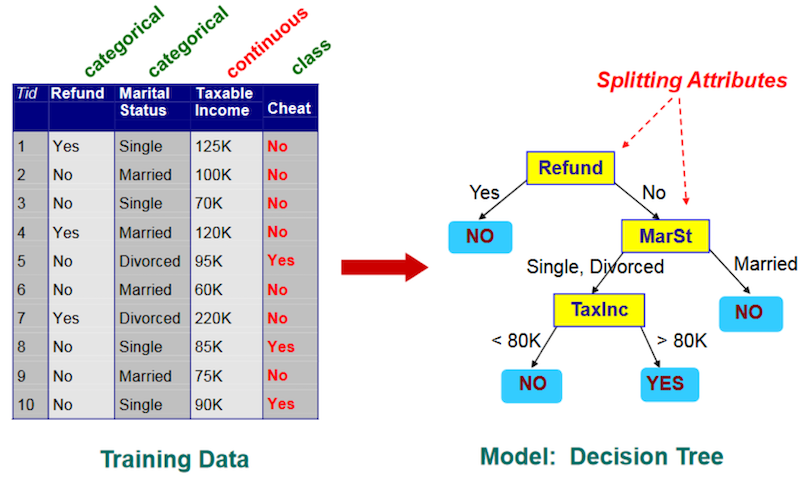
\includegraphics[scale=0.8]{figures/decision_tree_simple}
	\caption{Decision Tree simples Beispiel}
	\label{fig:dt_simple}
\end{figure}

Um einen Decision Tree erstellen zu können muss erst das Folgende geklärt werden:
\begin{itemize}
	\item Bestimmen wie die Samples aufgeteilt werden
	\begin{itemize}
		\item \textbf{Welche Attribute} (Features) sollen wann zum Splitten verwendet werden?
		\item Wie bestimmen wir den \textbf{besten} Split?
		\item Wie bestimmen wir die \textbf{Bedingung der Aufteilung}? Bspw. wenn Feature $x_{1} < 1$ ist.
		\item Verwenden wir einen \textbf{2er (2-way)} Split oder einen \textbf{multi-way} Split?
	\end{itemize} 
	\item Bestimme wann mit dem Splitten \textbf{aufgehört} wird (Stop-Kriterium).
\end{itemize} 

% ======
\subsubsection{Bestimmung der Aufteilung}

Grundsätzlich wollen wir bei jedem Knoten den höchsten Grad an Aufteilung (bezüglich der Klassen) erreichen. \\

Betrachten wir das Beispiel in Abbildung \ref{fig:dt_split_data}, in welchem anhand von Grösse, Gewicht und Arbeitsstelle das Geschlecht erkennt werden soll. Einfachheitshalber wurden jeweils binäre Werte verwendet.

\begin{figure}[h!]
	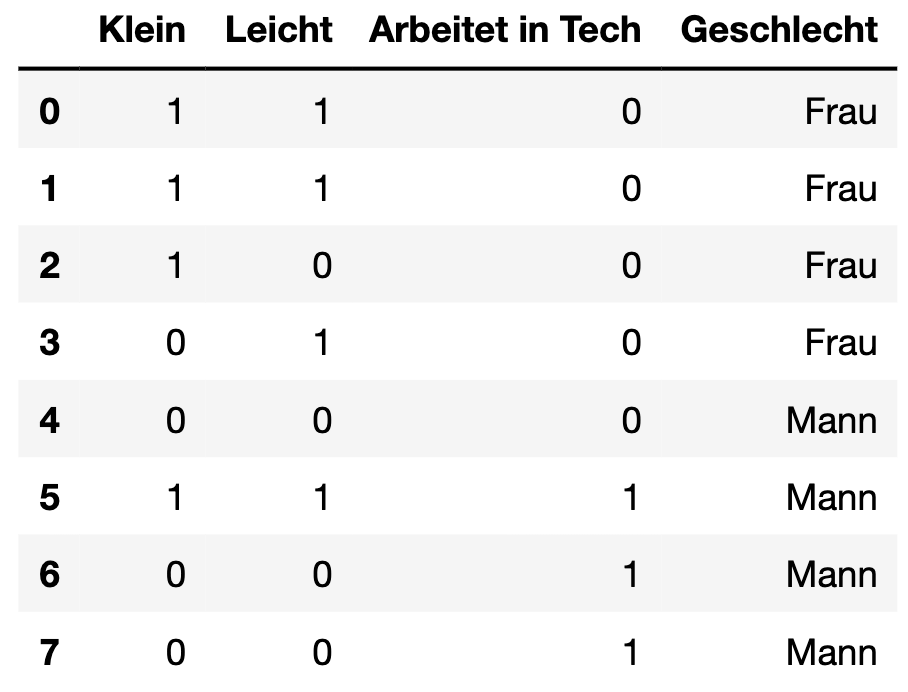
\includegraphics[scale=0.8]{figures/decision_tree_ex1_data}
	\caption{Decision Tree Beispiel Aufteilung Daten}
	\label{fig:dt_split_data}
\end{figure}

Nun stellt sich die Frage welches Feature (klein, leicht, Arbeitet in Tech) für die erste Entscheidung des Decision Trees verwendet werden soll. Also bspw. ist die Person klein? \\

Dafür rechnet der DT für jedes Feature (für jede möglich Decision) den \textbf{Information Gain} mit Hilfe der \textbf{Entropy} aus. \\

In Abbildung \ref{fig:dt_split} ist der DT zum obigen Beispiel. Man beachte, dass jeweils die Entropy der Knoten angezeigt wird.


\newpage
\begin{figure}[h!]
	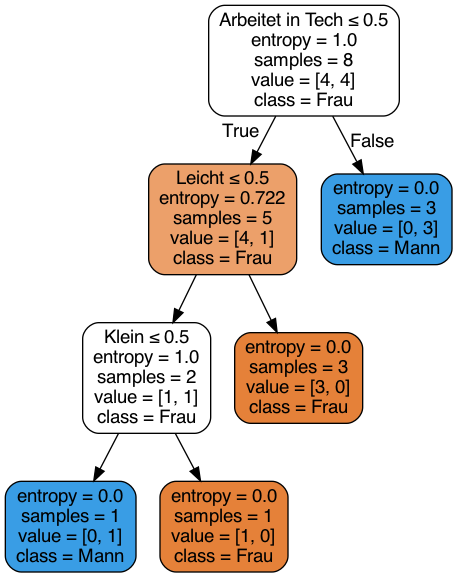
\includegraphics[scale=0.6]{figures/decision_tree_ex1}
	\caption{Decision Tree Beispiel Aufteilung}
	\label{fig:dt_split}
\end{figure}

Die \textbf{Entropy} eines einzelnen Knoten rechnet sich wie folgt:
$$ H(X) = - \sum_{c \in C} p_{c} * log_{2}(p_{c}) $$

\begin{align*}
	H(X) &= \text{Entropy des Datensets X} \\
	C &= \text{Menge der Target-Klassen (bspw. {Mann, Frau})} \\
	p_{c} &= \text{Wahrscheinlichkeit der Klasse c} \\
	      &= \frac{\text{Anzahl Samples der Klasse c}}{\text{Grösse des betrachteten Datensets}}  \\
\end{align*}

Beim ersten Knoten des DT haben wir 8 Samples ($|X| = 8$) und jeweils vier Männer und vier Frauen. Somit:

$$ H(X) = -\left(\frac{4}{8} * log_{2}\left(\frac{4}{8}\right) + \frac{4}{8} * log_{2}\left(\frac{4}{8}\right)\right) = 1 $$


Beim zweiten inneren Knoten des DT haben wir noch 5 Samples ($|X| = 5$) bestehend aus vier Frauen und einem Mann. Somit:

$$ H(X) = -\left(\frac{4}{5} * log_{2}\left(\frac{4}{5}\right) + \frac{1}{5} * log_{2}\left(\frac{1}{5}\right)\right) = 0.722 $$



Der untere Graph stellt die Funktion $H(X)$ für zwei Klassen dar. Die  Entropy kann auch als \textbf{Unordnung / Mix aus Klassen} betrachtet werden.

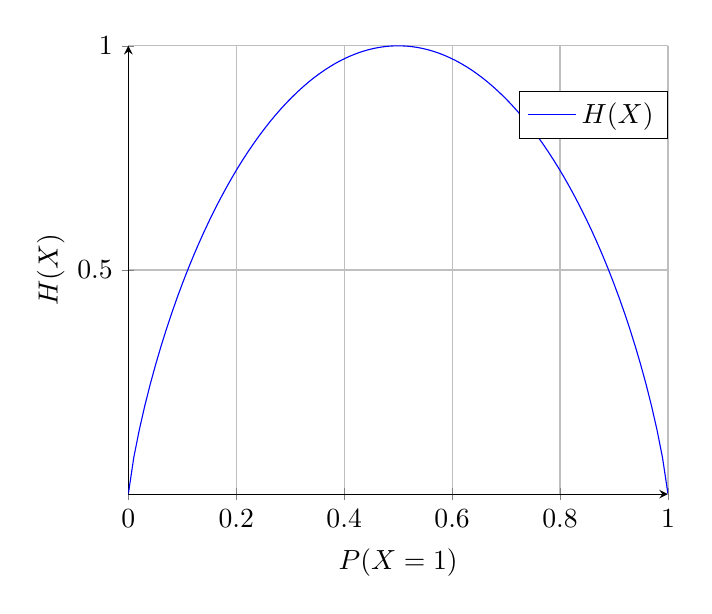
\begin{tikzpicture}[declare function={H(\x)=-1*(\x*log2{\x} + (1-\x)*log2{(1-\x)});}]
\begin{axis}%
[
    grid=major,     
    xmin=0,
    xmax=1,
    axis x line=bottom,
    ytick={0,.5,1},
    ymax=1,
    axis y line=middle,
    samples=100,
    domain=0:1,
    legend style={at={(1,0.9)}},
    x label style={at={(axis description cs:0.5,-0.1)},anchor=north},
    y label style={at={(axis description cs:-0.1,.5)},rotate=90,anchor=south},
    ylabel={$H(X)$},
    xlabel={$P(X=1)$}
]
    \addplot[blue,mark=none]   (x,{H(x)});
    \legend{$H(X)$}
\end{axis}
\end{tikzpicture}

Besteht $X$ nur aus einer Klasse so ist die Entropy 0. Sind beide Klassen gleich oft in $X$ vertreten, ist die Entropy maximal ($H(X) = 1$). Umso grösser die Entropy ist, desto grösser die \textbf{Unordnung} bezüglich der Klassen im Datenset.\\


Nun da wir wissen wie die Entropy berechnet wird, können wir uns der \textbf{Bestimmung der Aufteilung} widmen. Wir gehen wie folgt vor:

\begin{itemize}
	\item Berechnen der Entropy \textbf{vor und nach einem potentiellen Split}.
	\item Der Split, welcher die \textbf{Unordnung (Entropy) am meisten reduziert} wird priorisiert.
\end{itemize}


Bei unserem Beispiel haben wir drei Möglichkeiten für den ersten Split:
\begin{itemize}
	\item Ist die Person klein?
	\item Ist die Person leicht?
	\item Arbeitet die Person in einem Tech-Umfeld?
\end{itemize}
Dafür rechnen wir für jeden möglichen Split den \textbf{Information Gain} aus.
$$ \textbf{Information Gain} = \text{Entropy des Parent Node} - \text{Durchschnitt der Entropy der child-nodes} $$

\newpage

Die Entropy der Parent Nodes ist jeweils 1 wie wir bereits zuvor gezeigt haben. \\

\textbf{Ist die Person (nicht) klein?}
\begin{figure}[H]
	\centering
	\begin{forest}
	for tree={
		draw, 
		s sep=3em,
		parent anchor=south,
        child anchor=north,
        align=center,
        inner sep=1pt,
	}
	[klein $\leq 0.5$ \\ \text{Entropy = 1} \\ \text{\textbar X\textbar = 8 (Frau:4, Mann:4)}
	    [\text{Entropy = 0.811} \\ \text{\textbar X\textbar = 4 (Frau:1, Mann:3)}]
	    [\text{Entropy = 0.811} \\ \text{\textbar X\textbar = 4 (Frau:3, Mann:1)}]
	]
	\end{forest}
\end{figure}

Entropy der Child-Nodes ist jeweils:
$$ H(X) = -\left(\frac{1}{4} * log_{2}\left(\frac{1}{4}\right) + \frac{3}{4} * log_{2}\left(\frac{3}{4}\right)\right) = 0.811 $$

Der Information Gain:

$$ 1 - \frac{1}{2}*(0.811 + 0.811) = 0.189 $$

\textbf{Ist die Person (nicht) leicht?}
\begin{figure}[H]
	\centering
	\begin{forest}
	for tree={
		draw, 
		s sep=3em,
		parent anchor=south,
        child anchor=north,
        align=center,
        inner sep=1pt,
	}
	[klein $\leq 0.5$ \\ \text{Entropy = 1} \\ \text{\textbar X\textbar = 8 (Frau:4, Mann:4)}
	    [\text{Entropy = 0.811} \\ \text{\textbar X\textbar = 4 (Frau:1, Mann:3)}]
	    [\text{Entropy = 0.811} \\ \text{\textbar X\textbar = 4 (Frau:3, Mann:1)}]
	]
	\end{forest}
\end{figure}

Entropy der Child-Nodes ist jeweils:
$$ H(X) = -\left(\frac{1}{4} * log_{2}\left(\frac{1}{4}\right) + \frac{3}{4} * log_{2}\left(\frac{3}{4}\right)\right) = 0.811 $$

Der Information Gain:

$$ 1 - \frac{1}{2}*(0.811 + 0.811) = 0.189 $$


\newpage
\textbf{Arbeitet die Person (nicht) in Tech?}
\begin{figure}[H]
	\centering
	\begin{forest}
	for tree={
		draw, 
		s sep=3em,
		parent anchor=south,
        child anchor=north,
        align=center,
        inner sep=1pt,
	}
	[arbeitet in Tech $\leq 0.5$ \\ \text{Entropy = 1} \\ \text{\textbar X\textbar = 8 (Frau:4, Mann:4)}
	    [\text{Entropy = 0.722} \\ \text{\textbar X\textbar = 5 (Frau:4, Mann:1)}]
	    [\text{Entropy = 0} \\ \text{\textbar X\textbar = 3 (Frau:0, Mann:3)}]
	]
	\end{forest}
\end{figure}

Entropy des linken Child-Nodes ist:
$$ H(X) = -\left(\frac{4}{5} * log_{2}\left(\frac{4}{5}\right) + \frac{1}{5} * log_{2}\left(\frac{1}{5}\right)\right) = 722 $$

Entropy des rechten Child-Nodes ist:
$$ H(X) = -\left(0 + \frac{3}{3} * log_{2}\left(\frac{3}{3}\right)\right) = 0 $$

Der Information Gain:

$$ 1 - \frac{1}{2}*(0 + 0.722) = 0.639 $$

Den Split auf diesem Feature gibt uns also den höchsten Information Gain (reduziert die Unordnung im Datenset am Meisten). Daher wurde dieses Feature vom DT in Abbildung \ref{fig:dt_split} gewählt. \\

Diese Verfahren würde nun für die verbleibenden Samples im linken Child-Node weitergeführt werden.

% =========
\newpage
\subsubsection{Aufteilungsarten}

Die Aufteilung einer Decision kann in zwei Arten erfolgen. 

\textbf{multi-way split:}\\
\begin{figure}[H]
	\centering
	\label{fig:dt_multi}
	\begin{forest}
	for tree={draw, s sep=3em}
	[Car Type
	    [Family]
	    [Sports]
	    [Luxury]
	]
	\end{forest}
	\caption{Decision Tree multi-way Splitt}
\end{figure}


\textbf{2-way split (binär):}\\
Diese Variante wird meistens verwendet und ist einfacher zu optimieren.

\begin{figure}[H]
	\centering
	\label{fig:dt_binary}
	\begin{forest}
	for tree={draw, s sep=3em}
	[Car Type Family?
	    [Family]
	    [Car Type
	    	[Sports]
	    	[Luxury]
	    ]
	]
	\end{forest}
	\caption{Decision Tree 2-way Splitt}
\end{figure}


\subsubsection{Stop Kriterium}

Im idealen Fall sind nach einigen Entscheidungen nur noch Samples derselben Klasse in einem Branch übrig.  Jedoch ist dies in der Praxis selten der Fall. \\

Aus diesem Grund müssen wir definieren, wann der DT mit der Aufteilung (erstellen neuer internal nodes) aufhören soll. Dafür dient der \textbf{Hunt's} Algorithmus. \\

Dieser nutzt die folgenden Stop-Kriterien beim Erstellen des Baumes.

\begin{itemize}
	\item Alle Samples in einem Knoten gehören derselben Klasse an.
	\item Alle Samples in einem Knoten haben ähnliche Attribute (Features).
	\item Eine minimale (zuvor spezifizierte) Anzahl an Samples sind in einem Knoten vorhanden.
\end{itemize}

Die letzte Bedingung sorgt dafür, dass wir nicht einen riesigen Baum erstellen, welcher schlussendlich je nur ein Sample pro externen Knoten hat.

\newpage
\subsection{Vor und Nachteile des Decision Trees}

\subsubsection{Vorteile}

\begin{itemize}
	\item \textbf{Interpretierbar}
	\begin{itemize}
		\item Kann mathematisch zu 100 Prozent nachvollzogen werden warum wann welche Decision getroffen wird.
		\item Neue (ungesehene) Samples könnten von Hand durch die Entscheidungen des Trees durchlaufen werden. (quasi \textbf{manuelles debugging}).
	\end{itemize}
	\item \textbf{Skalierbar}
	\begin{itemize}
		\item Durch Verwendung des Hunt's Algo
		\item Funktioniert auch für eine sehr grosse Anzahl Features gut.
		\item Gute Geschwindigkeit des Lernens und Verarbeiten von Samples
	\end{itemize}
	\item \textbf{Einfach zu implementieren}
\end{itemize}


\subsubsection{Nachteile}

Der grösste und schwerwiegendste Nachteil des Decision Trees ist die Tendenz zum \textbf{Overfitting}. \\

Umso grösser der Tree wird (mehr Knoten) desto schlechter wird die Genauigkeit auf neuen Daten. Abbildung \ref{fig:dt_overfitting} zeigt die zunehmende Kluft die sich zwischen Training- und Testdaten ergibt.

\begin{figure}[h!]
	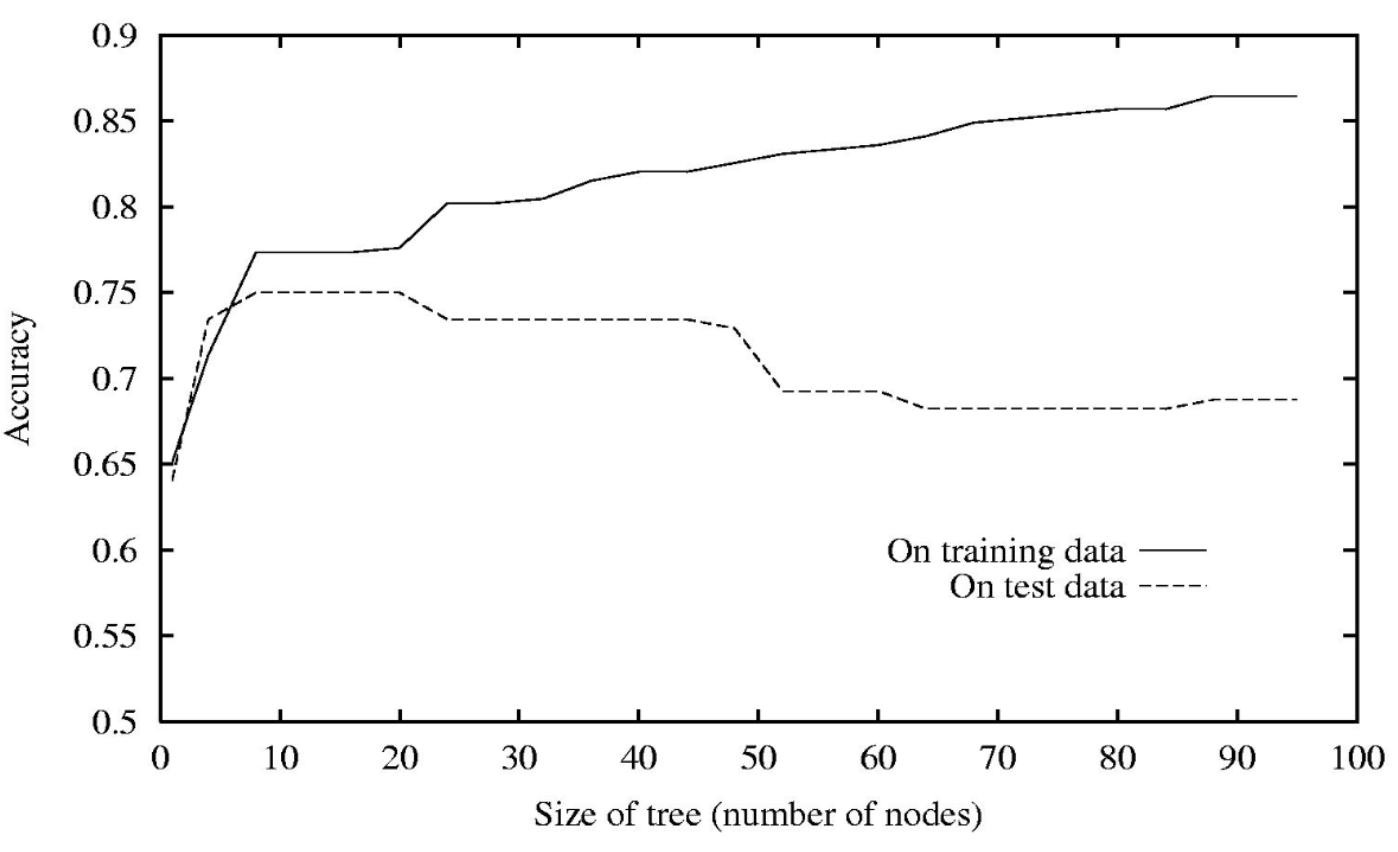
\includegraphics[scale=0.6]{figures/decision_tree_overfitting}
	\caption{Decision Tree Overfitting}
	\label{fig:dt_overfitting}
\end{figure}

\newpage
\subsubsection{Overfitting verhindern}

Um die Kluft zwischen Training- und Testdaten bezüglich der Genauigkeit zu verhindern, können diese Strategien angewendet werden: \\

\textbf{Limitieren der Tiefe (Anzahl Layer im Tree)}\\
Dies zwingt den DT Attribute zu verwenden, die über das ganze Datenset hinweg charakteristische Relevanz haben. Und \textbf{nicht} Attribute verwenden, die nur für sehr wenige Samples zutreffen.



\textbf{Eine minimale Anzahl Samples per externen Knoten fordern}\\
Verfolgt das gleiche Ziel wie oben, jedoch ohne explizit die Tiefe zu Limitieren. Da in jedem externen Knoten eine Mindestanzahl gefordert wird, kann der DT keine all zu spezifischen Decisions definieren.

